\begin{blocksection}
\textbf{\underline{5 Stages of a Single Cycle CPU:}}

\begin{itemize}
    \item Instruction Fetch (IF) - Fetch from memory (IMEM) 
    \item Instruction Decode (ID) - Decode instruction
    \item Execute (EX) - Execute operation (arithmetic, shifting, etc) using ALU
    \item Memory Access (MEM) - Load and store instructions access memory
    \item Write Back to Register (WB) - Write instruction back to RegFile
\end{itemize}
\bigskip
\textbf{\underline{Datapaths: A Visual Approach}}

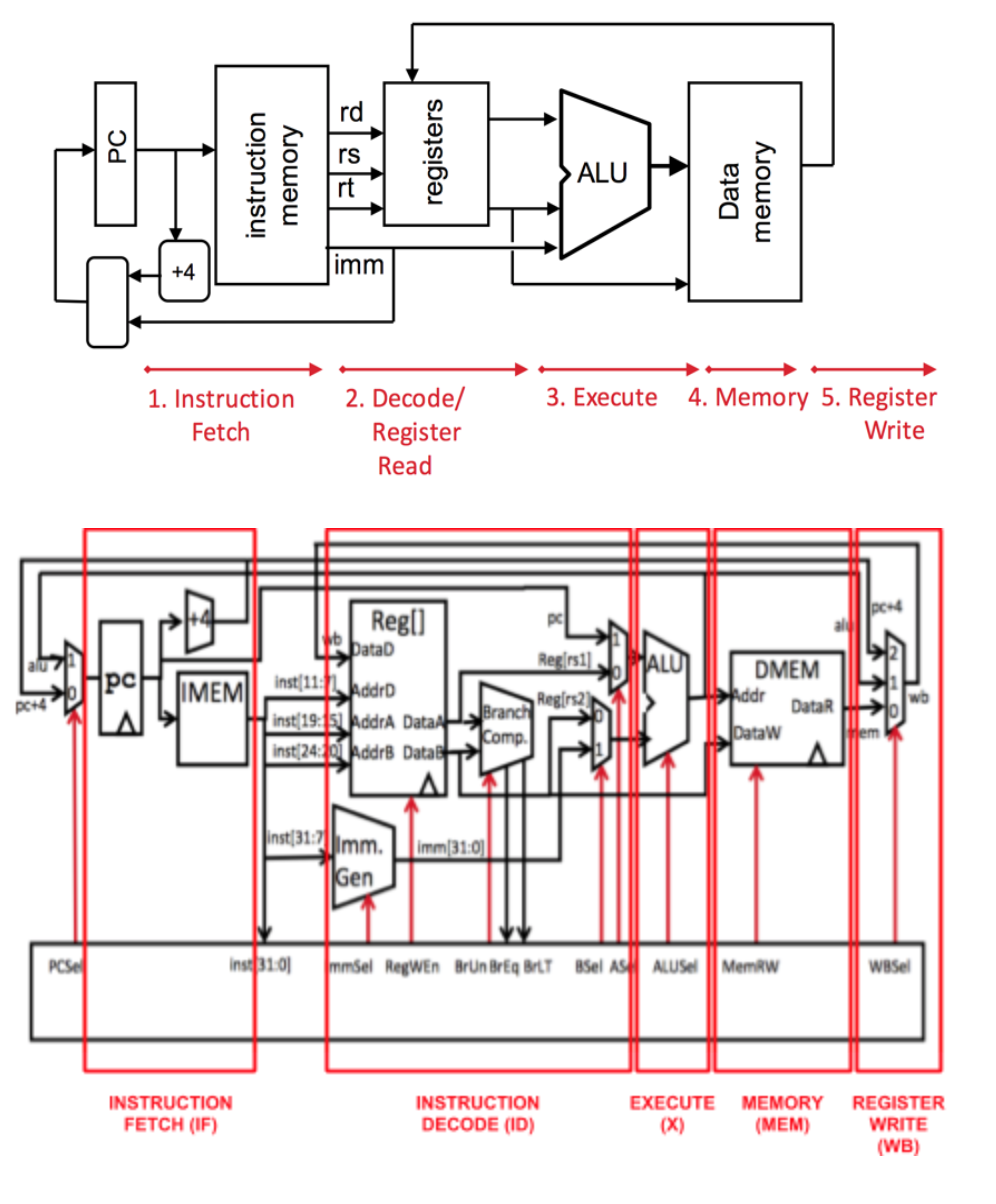
\includegraphics[width=\textwidth]{singlecycle/explanation_1}

\end{blocksection}